%!TEX root = ../rsra.tex

\chapter{Availability and Maintainability}
\section{Introduction}
\emph{Can I repair the system after a failure?} We can classify systems into two
categories according to the answer to this question.
\begin{itemize}
    \item \textbf{Non maintained systems} These systems cannot be repaired after a
    failure (e.g. a  telecommunication satellite, a F1 engine, a vessel of a nuclear
    power plant).
    
    $\to$ a good \emph{performance parameter} is the \emph{reliability}, as it
    quantifies the system capability of satisfying a specified mission within an
    assigned period of time ($T_M$): $R(T_M) = P(T>T_M)$

    \item \textbf{Maintained systems} These systems can be repaired after the failure
    (e.g. pump of an energy production plant, a component of the reactor emergency
    cooling systems).
    
    $\to$ a good \emph{performance parameter} is the \emph{availability}, as it
    quantifies the system ability to fulfill the assigned mission at any specific
    moment in the lifetime: $A(t)$.
\end{itemize}

We will now try to give now a more rigorous definition of \emph{availability}.

\section{Definition of Availability}
Let's tackle the problem from a mathematical point of view.

We introduce an indicator variable $X(t)$ such that:
\begin{equation*}
    X(t)=\begin{cases}
        1 & \text{system is operating at time } t \\
        0 & \text{system is failed at time } t
    \end{cases}
\end{equation*}

\begin{figure}[!htp]
    \centering
    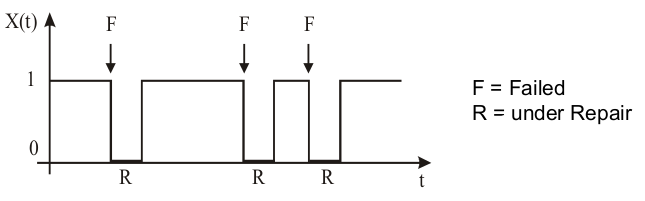
\includegraphics[width=.85\textwidth]{x(t)_example.png}
    \caption{An example of $X(t)$ for a given system}
\end{figure}

\subsection{Instantaneous availability}
\begin{equation*}
    p(t) = P\{X(t)=1\} = E[X(t)]
\end{equation*}

Notice that:
\begin{equation*}
    E[X(t)] = \sum_{i=0}^1 iP\{X(t)=i\} = 0\cdot P\{X(t)=0\} + 1\cdot P\{X(t)=1\} = p(t)
\end{equation*}

\subsection{Instantaneous unavailability}
\begin{equation*}
    q(t) = P\{X(t) = 0\} = 1 - p(t)
\end{equation*}
where the last equivalence comes from the fact that the two events "system is
operating at time t" and "system is failed at time t" are mutually exclusive.

\section{Contributions to Unavailability}
\subsection{Repair}
A component can be unavailable because it is under repair after a failure.

\subsection{Testing / Preventive Maintenance}

\subsection{Unrevealed failure}

\section{Average availability descriptors}